%%%%%%%%%%%%%%%%%%%%%%%%%%%%%%%%%%%%%%%%%%%%%%%%%%%%%%%%%%%%%%%%%%%%%%%%%%%%%%%%%%
\begin{frame}[fragile]\frametitle{}
\begin{center}
{\Large Concepts}
\end{center}
\end{frame}

%%%%%%%%%%%%%%%%%%%%%%%%%%%%%%%%%%%%%%%%%%%%%%%%%%%%%%%%%%%%%%%%%%%%%%%%%%%%%%%%%%
\begin{frame}[fragile]\frametitle{Example}


\begin{itemize}
\item A robot looks at boxes on a conveyor belt and segregates them into Good or Bad bins based on their weight.
\item What's the Environment, Action, Agent and Reward here?

\end{itemize}

\begin{center}
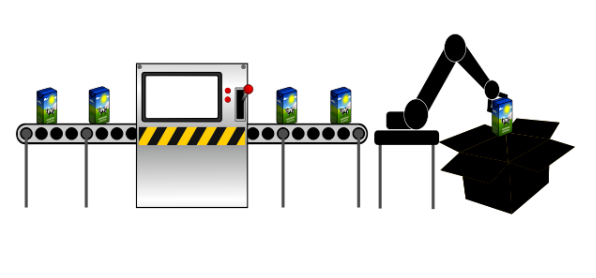
\includegraphics[width=0.8\linewidth,keepaspectratio]{rl68}
\end{center}

{\tiny (Ref: Modern Reinforcement Learning: Deep Q Learning in PyTorch - Phil Tabor)}

\end{frame}

%%%%%%%%%%%%%%%%%%%%%%%%%%%%%%%%%%%%%%%%%%%%%%%%%%%%%%%%%%%%%%%%%%%%%%%%%%%%%%%%%%
\begin{frame}[fragile]\frametitle{Core Concepts in the Example}


\begin{itemize}
\item Agent is whoever acts: Robot's memory of (states, actions, rewards)
\item Environment: What changes when Agent (Robot) acts upon? : Boxes. Position of the boxes change and Rewards given to the agent/robot. So, Environment = Boxes + Rewards. Btw, Rewards are always with Environment.
\item Reward, indicator that heps decision: Good/Bad
\item State: Reading on the weight sensor.State space is the range of weights possible.
\item Action: Discrete (move to good/bad bin), causes new box to load, then new weight happens. Q Learning works on Discrete spaces like this but for continuous spaces algorithms like Actor-Critique are used.
\end{itemize}

\begin{center}
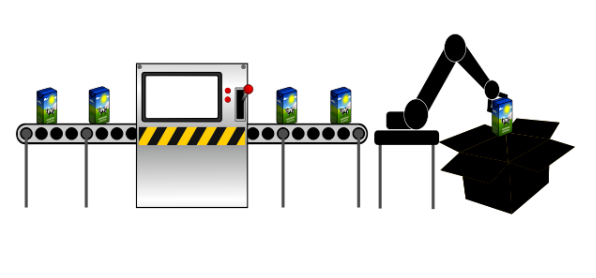
\includegraphics[width=0.4\linewidth,keepaspectratio]{rl68}
\end{center}

{\tiny (Ref: Modern Reinforcement Learning: Deep Q Learning in PyTorch - Phil Tabor)}

\end{frame}

%%%%%%%%%%%%%%%%%%%%%%%%%%%%%%%%%%%%%%%%%%%%%%%%%%%%%%%%%%%%%%%%%%%%%%%%%%%%%%%%%%
\begin{frame}[fragile]\frametitle{Environment}


\begin{center}
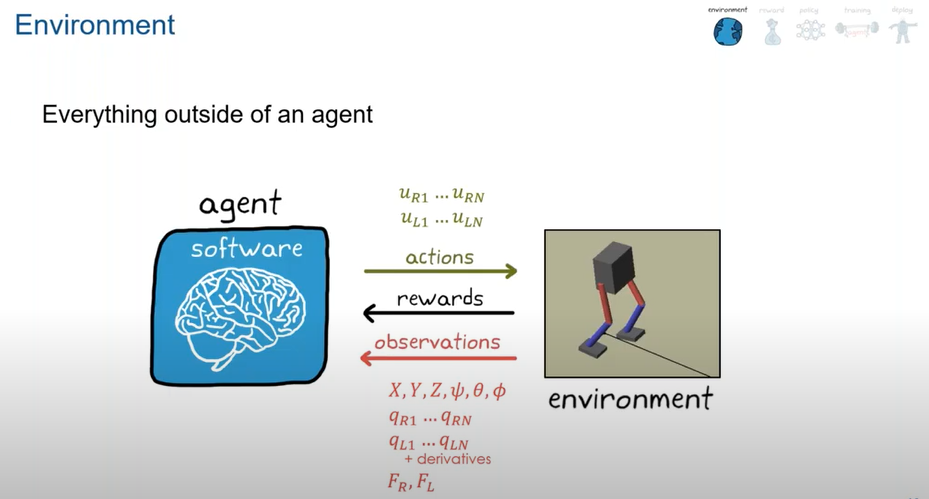
\includegraphics[width=0.9\linewidth,keepaspectratio]{rl76}
\end{center}

{\tiny (Ref: How to Train Your Robot: An Introduction to Reinforcement Learning - Craig Buhr PhD)}

\end{frame}

%%%%%%%%%%%%%%%%%%%%%%%%%%%%%%%%%%%%%%%%%%%%%%%%%%%%%%%%%%%%%%%%%%%%%%%%%%%%%%%%%%
\begin{frame}[fragile]\frametitle{Real vs Simulated Environment}


\begin{center}
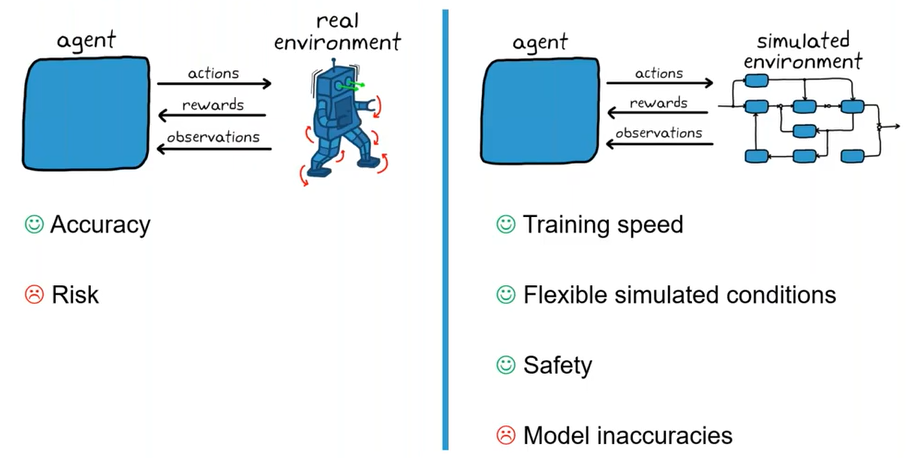
\includegraphics[width=0.9\linewidth,keepaspectratio]{rl77}
\end{center}

{\tiny (Ref: How to Train Your Robot: An Introduction to Reinforcement Learning - Craig Buhr PhD)}

\end{frame}

%%%%%%%%%%%%%%%%%%%%%%%%%%%%%%%%%%%%%%%%%%%%%%%%%%%%%%%%%%%%%%%%%%%%%%%%%%%%%%%%%%
\begin{frame}[fragile]\frametitle{Reward}


\begin{center}
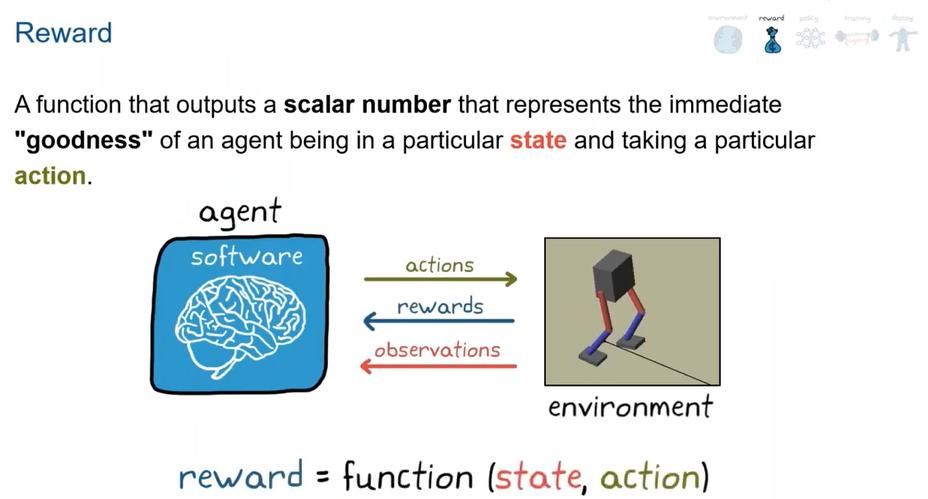
\includegraphics[width=0.9\linewidth,keepaspectratio]{rl78}
\end{center}

{\tiny (Ref: How to Train Your Robot: An Introduction to Reinforcement Learning - Craig Buhr PhD)}

\end{frame}

%%%%%%%%%%%%%%%%%%%%%%%%%%%%%%%%%%%%%%%%%%%%%%%%%%%%%%%%%%%%%%%%%%%%%%%%%%%%%%%%%%
\begin{frame}[fragile]\frametitle{Defining Reward}

For Robot walking in straight line, it should not fall, be fast, etc.

\begin{center}
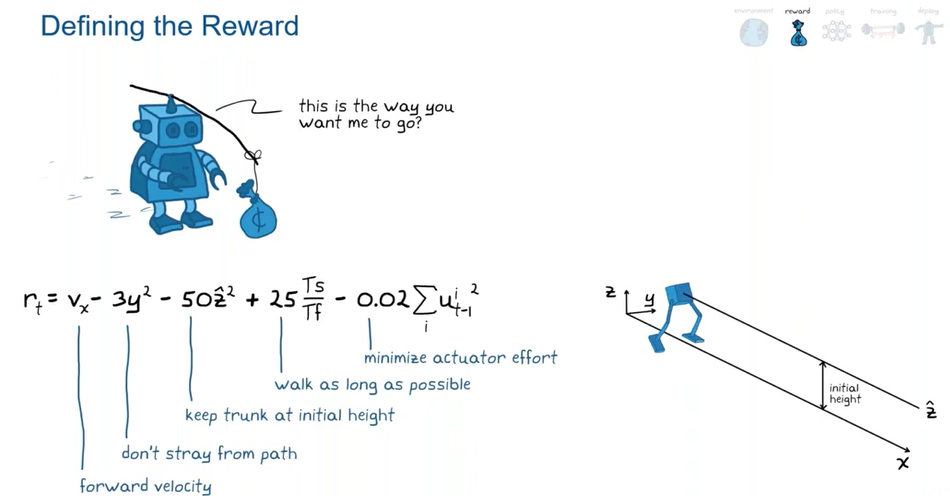
\includegraphics[width=0.9\linewidth,keepaspectratio]{rl79}
\end{center}

{\tiny (Ref: How to Train Your Robot: An Introduction to Reinforcement Learning - Craig Buhr PhD)}

\end{frame}



%%%%%%%%%%%%%%%%%%%%%%%%%%%%%%%%%%%%%%%%%%%%%%%%%%%%%%%%%%%%%%%%%%%%%%%%%%%%%%%%%%
\begin{frame}[fragile]\frametitle{Basic Entities}


\begin{itemize}
\item Agent : Entity learning about the environment and making decisions. We need to specify a learning algorithm for the agent that allows it to learn a policy
\item Environment: Everything outside the agent, including other agents
\item Rewards: Numerical quantities that represent feedback from the environment that an agent tries to maximize
\item State: A representation of the environment. At time step $t$,the agent is in state $S_t \in S$ where $S$ is the set of all possible states
\item Action: At time step $t$, an agent takes an action $A_t \in A(S_t)$ where $A(S_t)$ is the set of actions available in state $S_t$
\item Policy: A policy tells the agent what action to take in a given state $\pi(a|S)$. A policy can be deterministic i.e. there is one action that is deterministically selected in a given state $\pi(s)=a$, or stochastic i.e. the policy maps a state onto a set of probabilities for taking each action. $p(a_i|s) < 1$ subject to $\sum_{i} p(a_i|s) = 1$
\item To solve a problem using RL, we should be able to formulate it as a Markov Decision Process (MDP).
\end{itemize}



{\tiny (Ref: Solving Tic-Tac-Toe with Reinforcement Learning - Govind G Nair)}

\end{frame}

%%%%%%%%%%%%%%%%%%%%%%%%%%%%%%%%%%%%%%%%%%%%%%%%%%%%%%%%%%%%%%%%%%%%%%%%%%%%%%%%%%
\begin{frame}[fragile]\frametitle{MDP}


\begin{itemize}
\item In an MDP, the environment is completely characterized by the transition dynamics equation $p(s',r|s,a)$.
\item That is, the probability of each possible value for $s'$ (the subsequent state) and $r$ (reward) depends only on the immediately preceding state and action,$s$ and $a$, and, given them, not at all on earlier states and actions. In other words, given the present, the future is independent of the past.
\item The state must include information about all aspects of the past agent–environment interaction that make a difference for the future. If it does, then the state is said to have the Markov property
\item If the transition dynamics equation is fully known by the agent, it means an optimal policy can be computed without interacting with the environment. This is planning. Some kind of search algorithm can be used here.
\item When the environment is not fully known, the agent has to learn by interacting with the environment. i.e. learning. If an agent constructs a model of the environment , it is called model based RL, else it is called model free RL.
\end{itemize}



{\tiny (Ref: Solving Tic-Tac-Toe with Reinforcement Learning - Govind G Nair)}

\end{frame}

%%%%%%%%%%%%%%%%%%%%%%%%%%%%%%%%%%%%%%%%%%%%%%%%%%%%%%%%%%%%%%%%%%%%%%%%%%%%%%%%%%
\begin{frame}[fragile]\frametitle{Path}


\begin{itemize}
\item When an agent in state $s_t$ takes an action $A_t$ as prescribed by a policy $\pi$ , it transitions to a state $s_{t+1}$ and receives a reward $R_{t+1}$. The Agent interacting with the ``MDP'' environment thus gives rise to a sequence or trajectory $S_0,A_0,R_1,S_1,A_1,R_2,S_2,\ldots$
\item The goal of an agent is to maximize the long term reward or return.
\item Long term reward or return is formally defined as the discounted sum of future rewards. $G_t = R_{t+1} + \gamma R_{t+2} + \gamma R_{t+3} + \ldots = \sum_{k=0}^{\infty} \gamma^k R{t+k+1} = R_{t+1} + \gamma G_{t+1}$
\end{itemize}



{\tiny (Ref: Solving Tic-Tac-Toe with Reinforcement Learning - Govind G Nair)}

\end{frame}


%%%%%%%%%%%%%%%%%%%%%%%%%%%%%%%%%%%%%%%%%%%%%%%%%%%%%%%%%%%%%%%%%%%%%%%%%%%%%%%%%%
\begin{frame}[fragile]\frametitle{Model}


\begin{itemize}
\item Defines the reward function and transition probabilities.
\item {\bf Know the model}: planning with perfect information; do model-based RL. When we fully know the
environment, we can find the optimal solution by Dynamic Programming (DP).
\item {\bf Do not know the model}: planning with perfect information; do model-based RL. When we fully know the
environment, we can find the optimal solution by Dynamic Programming (DP).
\end{itemize}


\begin{center}
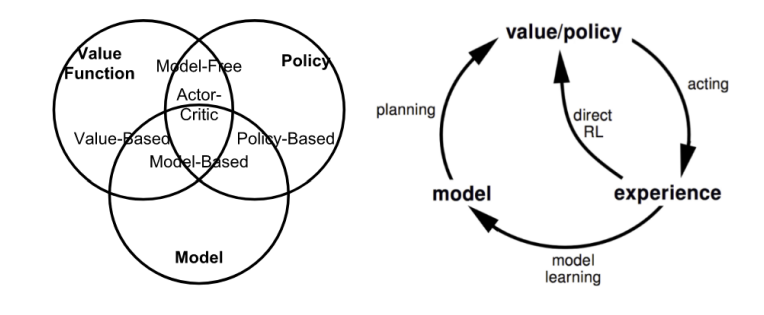
\includegraphics[width=0.8\linewidth,keepaspectratio]{rl98}
\end{center}


{\tiny (Ref: A (Long) Peek into Reinforcement Learning - Lilian Weng)}


\end{frame}

%%%%%%%%%%%%%%%%%%%%%%%%%%%%%%%%%%%%%%%%%%%%%%%%%%%%%%%%%%%%%%%%%%%%%%%%%%%%%%%%%%
\begin{frame}[fragile]\frametitle{Approaches}


\begin{itemize}
\item Model-based: Rely on the model of the environment; either the model is known or the algorithm learns it explicitly.
\item Model-free: No dependency on the model during learning.
\item On-policy: Use the deterministic outcomes or samples from the target policy to train the algorithm.
\item Off-policy: Training on a distribution of transitions or episodes produced by a different behavior
policy rather than that produced by the target policy.
\end{itemize}

{\tiny (Ref: A (Long) Peek into Reinforcement Learning - Lilian Weng)}


\end{frame}

%%%%%%%%%%%%%%%%%%%%%%%%%%%%%%%%%%%%%%%%%%%%%%%%%%%%%%%%%%%%%%%%%%%%%%%%%%%%%%%%%%
\begin{frame}[fragile]\frametitle{Model: Transition and Reward}


\begin{itemize}
\item The model is a descriptor of the environment. 
\item With the model, we can learn or infer how the
environment would interact with and provide feedback to the agent. 
\item The model has two major parts, transition probability function $P$ and reward function $R$.
\item The transition function $P$ records the probability of transitioning from state $s$ to $s'$ after taking action $a$
while obtaining reward $r$. ie $P(s',r|s,a)=P[S_{t+1} = s',R_{t+1} = r|S_t = s, A_t = a]$
\item The reward function R predicts the next reward triggered by one action: $R(s,a) = E[R_{t+1} |S_t = s, A_t = a] = \sum_{r \in R} r \sum_{s' \in S}P(s',r|s,a)$
\end{itemize}

{\tiny (Ref: A (Long) Peek into Reinforcement Learning - Lilian Weng)}


\end{frame}

%%%%%%%%%%%%%%%%%%%%%%%%%%%%%%%%%%%%%%%%%%%%%%%%%%%%%%%%%%%%%%%%%%%%%%%%%%%%%%%%%%
\begin{frame}[fragile]\frametitle{Policy}

Policy, as the agent’s behavior function  , tells us which action to take in state s. It is a mapping from
state s to action a and can be either 

\begin{itemize}
\item Deterministic: $\pi(s)=a$, also denoted as $\mu(s_t)=a_t$
\item Stochastic: $\pi (a|s) = P_{\pi}[A=a|S=a]$
\end{itemize}

{\tiny (Ref: A (Long) Peek into Reinforcement Learning - Lilian Weng)}

\end{frame}

%%%%%%%%%%%%%%%%%%%%%%%%%%%%%%%%%%%%%%%%%%%%%%%%%%%%%%%%%%%%%%%%%%%%%%%%%%%%%%%%%%
\begin{frame}[fragile]\frametitle{Deep RL Policy}

Deep RL, 
\begin{itemize}

\item Has parameterized policies: policies whose outputs are computable functions that depend on a set of parameters (eg the weights and biases of a neural network) which we can adjust to change the behavior via some optimization algorithm.
\item Weights are denoted by $\theta$ or $\phi$, so equations become: $a_t=\mu_\theta(_t)$ or for stochastic $a_t \sim \pi_\theta(.|s_t)$
\end{itemize}

{\tiny (Ref: Spinning Up - Open AI)}


\end{frame}

%%%%%%%%%%%%%%%%%%%%%%%%%%%%%%%%%%%%%%%%%%%%%%%%%%%%%%%%%%%%%%%%%%%%%%%%%%%%%%%%%%
\begin{frame}[fragile]\frametitle{Deterministic Policy}

\begin{lstlisting}
pi_net = nn.Sequential(
              nn.Linear(obs_dim, 64),
              nn.Tanh(),
              nn.Linear(64, 64),
              nn.Tanh(),
              nn.Linear(64, act_dim)
            )
						
obs_tensor = torch.as_tensor(obs, dtype=torch.float32)
actions = pi_net(obs_tensor)
\end{lstlisting}

\end{frame}

%%%%%%%%%%%%%%%%%%%%%%%%%%%%%%%%%%%%%%%%%%%%%%%%%%%%%%%%%%%%%%%%%%%%%%%%%%%%%%%%%%
\begin{frame}[fragile]\frametitle{Stochastic  Policy}

Stochastic policies in deep RL: 
\begin{itemize}
\item categorical policies (discrete action spaces) 
\item diagonal Gaussian policies (continuous action spaces).
\end{itemize}

Two key computations:
\begin{itemize}
\item sampling actions from the policy,
\item and computing log likelihoods of particular actions, $\log \pi_{\theta}(a|s)$.
\end{itemize}

{\tiny (Ref: Spinning Up - Open AI)}
\end{frame}

%%%%%%%%%%%%%%%%%%%%%%%%%%%%%%%%%%%%%%%%%%%%%%%%%%%%%%%%%%%%%%%%%%%%%%%%%%%%%%%%%%
\begin{frame}[fragile]\frametitle{Trajectories}

\begin{itemize}
\item cA trajectory $\tau$ is a sequence of states and actions in the world, $\tau = (s_0, a_0, s_1, a_1, ...).$
\item The very first state of the world, $s_0$, is randomly sampled from the start-state distribution, sometimes denoted by $\rho_0$:
$s_0 \sim \rho_0(\cdot)$.
\item State transitions (what happens to the world between the state at time $t$, $s_t$, and the state at $t+1$, $s_{t+1}$, are governed by the natural laws of the environment, and depend on only the most recent action, $a_t$. They can be either:
\begin{itemize}
\item deterministic: $s_{t+1} = f(s_t, a_t)$
\item stochastic: $s_{t+1} \sim P(\cdot|s_t, a_t)$
\end{itemize}
\item Actions come from an agent according to its policy.
\item Trajectories are also frequently called episodes or rollouts.
\end{itemize}

{\tiny (Ref: Spinning Up - Open AI)}
\end{frame}

%%%%%%%%%%%%%%%%%%%%%%%%%%%%%%%%%%%%%%%%%%%%%%%%%%%%%%%%%%%%%%%%%%%%%%%%%%%%%%%%%%
\begin{frame}[fragile]\frametitle{The RL Problem}

For stochastic transitions and policy:

\begin{itemize}
\item probability of a $T$ -step trajectory is $P(\tau|\pi) = \rho_0 (s_0) \prod_{t=0}^{T-1} P(s_{t+1} | s_t, a_t) \pi(a_t | s_t).$
\item The expected return (for whichever measure), denoted by $J(\pi)$, is then: $J(\pi) = \int_{\tau} P(\tau|\pi) R(\tau) = E_{\tau\sim \pi}[R(\tau)]$.
\item The central optimization problem in RL can then be expressed by $\pi^* = \arg \max_{\pi} J(\pi),$
\item with $\pi^*$ being the optimal policy.
\end{itemize}

{\tiny (Ref: Spinning Up - Open AI)}
\end{frame}


%%%%%%%%%%%%%%%%%%%%%%%%%%%%%%%%%%%%%%%%%%%%%%%%%%%%%%%%%%%%%%%%%%%%%%%%%%%%%%%%%%
\begin{frame}[fragile]\frametitle{Value Function}


\begin{itemize}
\item Value function measures the goodness of a state or how rewarding a state or an action is by a
prediction of future reward. 
\item The future reward, also known as return, is a total sum of discounted rewards going forward. 
\item Let’s compute the return $G_t$ starting from time $t$: $G_t = R_{t+1} + \gamma R_{t+2} + \ldots = \sum_{k=0}^{\infty} \gamma^kR_{t+k+1}$
\item The future rewards may have higher uncertainty; i.e. stock market.
\item The future rewards do not provide immediate benefits; i.e. As human beings, we might prefer to
have fun today rather than 5 years later ;).
\item Discounting provides mathematical convenience; i.e., we don’t need to track future steps forever to
compute return.
\item We don’t need to worry about the infinite loops in the state transition graph.
\end{itemize}

{\tiny (Ref: A (Long) Peek into Reinforcement Learning - Lilian Weng)}
\end{frame}

%%%%%%%%%%%%%%%%%%%%%%%%%%%%%%%%%%%%%%%%%%%%%%%%%%%%%%%%%%%%%%%%%%%%%%%%%%%%%%%%%%
\begin{frame}[fragile]\frametitle{Main functions}

\begin{itemize}
\item The On-Policy Value Function, $V^{\pi}(s)$, which gives the expected return if you start in state s and always act according to policy $\pi$:$V^{\pi}(s) = E_{\tau \sim \pi}[R(\tau)\left| s_0 = s\right]$.
\item The On-Policy Action-Value Function, $Q^{\pi}(s,a)$, which gives the expected return if you start in state $s$, take an arbitrary action $a$ (which may not have come from the policy), and then forever after act according to policy $\pi$: $Q^{\pi}(s,a) = E_{\tau \sim \pi}[R(\tau)\left| s_0 = s, a_0 = a\right]$.
\item The Optimal Value Function, $V^*(s)$, which gives the expected return if you start in state $s$ and always act according to the optimal policy in the environment:
$V^*(s) = \max_{\pi} E_{\tau \sim \pi}[R(\tau)\left| s_0 = s\right]$.
\item The Optimal Action-Value Function, $Q^*(s,a)$, which gives the expected return if you start in state $s$, take an arbitrary action $a$, and then forever after act according to the optimal policy in the environment: $Q^*(s,a) = \max_{\pi} E_{\tau \sim \pi}[R(\tau)\left| s_0 = s, a_0 = a\right]$.
\end{itemize}

{\tiny (Ref: Spinning Up - Open AI)}
\end{frame}



%%%%%%%%%%%%%%%%%%%%%%%%%%%%%%%%%%%%%%%%%%%%%%%%%%%%%%%%%%%%%%%%%%%%%%%%%%%%%%%%%%
\begin{frame}[fragile]\frametitle{Main functions}

There are two key connections between the value function and the action-value function that come up pretty often:

\begin{itemize}
\item $V^{\pi}(s) = E_{a\sim \pi}[Q^{\pi}(s,a)]$,
\item $V^*(s) = \max_a Q^* (s,a).$
\end{itemize}

{\tiny (Ref: Spinning Up - Open AI)}
\end{frame}


%%%%%%%%%%%%%%%%%%%%%%%%%%%%%%%%%%%%%%%%%%%%%%%%%%%%%%%%%%%%%%%%%%%%%%%%%%%%%%%%%%
\begin{frame}[fragile]\frametitle{Components}


\begin{itemize}
\item 3 main components of RL: Q function, Policy function, model function
\item As deep learning can approximate any function over large state space it has become good representation learning for all 3 components. For small state space tables are ok but for large problems and continuous states like football field, function approximation is needed
\item How to evaluate a position? Let it play from there randomly till end with multiple ways, average them and that's the value. Monte Carlo tree search. Limited success.
\item Alpha go was with deep learning and not search

\end{itemize}

\end{frame}

%%%%%%%%%%%%%%%%%%%%%%%%%%%%%%%%%%%%%%%%%%%%%%%%%%%%%%%%%%%%%%%%%%%%%%%%%%%%%%%%%%
\begin{frame}[fragile]\frametitle{Observations vs States}

\begin{itemize}
\item Observation and State are different. Pixels of image are observation. State is what is there. Image is what is seen now. Observations result from state. Its like a view of underlying data.
\item Past observations give you additional information. But for states, being true, the last one is good enough.
\end{itemize}


\begin{center}
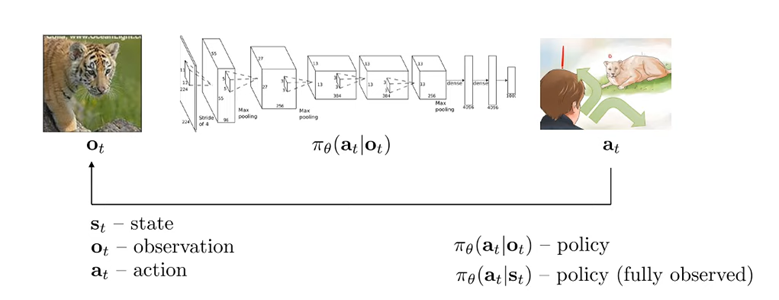
\includegraphics[width=0.7\linewidth,keepaspectratio]{rl48}
\end{center}


{\tiny (Ref: CS 285 Fall 2020 Deep Reinforcement Learning)}

\end{frame}

%%%%%%%%%%%%%%%%%%%%%%%%%%%%%%%%%%%%%%%%%%%%%%%%%%%%%%%%%%%%%%%%%%%%%%%%%%%%%%%%%%
\begin{frame}[fragile]\frametitle{Observations vs States}

\begin{itemize}
\item If you have observations, then past observations would be needed to find the truth (state), but if you have ready states then just the past/current one is good enough to decide the future action.
\item If predictions and data diverge, how to converge them? DAagger: Dataset Aggregation. Get data from predictions only. First train on human data, then run to predict, then have humans label the predictions/actions. Merge both datasets. Train on the whole dataset. Repeat to converge.
Conditions when Fit-the-expert strategy fails:
\begin{itemize}
\item Non-Markovian behavior: action depends not only on the past state but more. At same state actions are different.
\item 	Multimodal behavior: different streams of inputs decide the action.
\end{itemize}

\end{itemize}


\begin{center}
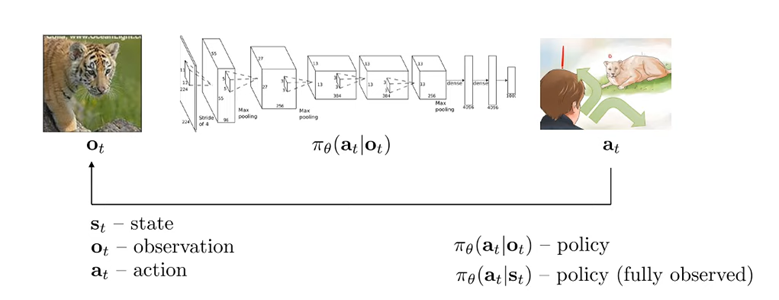
\includegraphics[width=0.7\linewidth,keepaspectratio]{rl48}
\end{center}


{\tiny (Ref: CS 285 Fall 2020 Deep Reinforcement Learning)}

\end{frame}

%%%%%%%%%%%%%%%%%%%%%%%%%%%%%%%%%%%%%%%%%%%%%%%%%%%%%%%%%%%%%%%%%%%%%%%%%%%%%%%%%%
\begin{frame}[fragile]\frametitle{How to learn Policy?}


\begin{center}
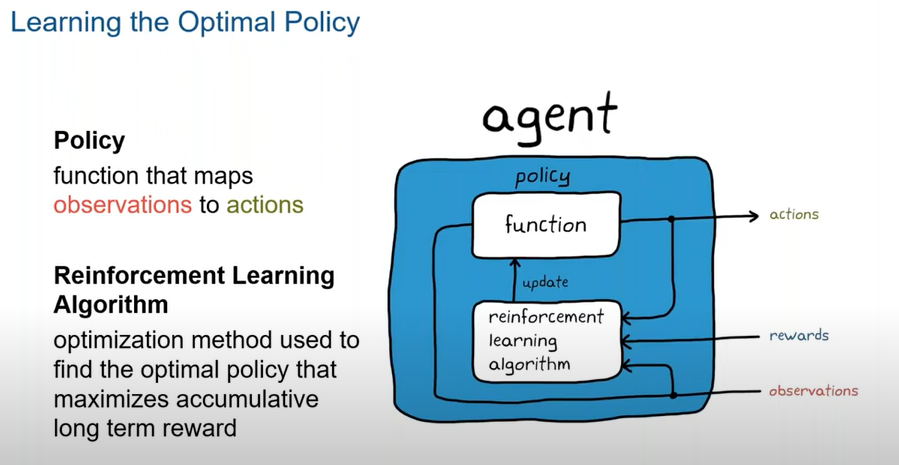
\includegraphics[width=0.9\linewidth,keepaspectratio]{rl75}
\end{center}

{\tiny (Ref: How to Train Your Robot: An Introduction to Reinforcement Learning - Craig Buhr PhD)}

\end{frame}


%%%%%%%%%%%%%%%%%%%%%%%%%%%%%%%%%%%%%%%%%%%%%%%%%%%%%%%%%%%%%%%%%%%%%%%%%%%%%%%%%%
\begin{frame}[fragile]\frametitle{How to learn Policy?}

Imitation Learning (behavior cloning): Take labelled data and do supervised learning. It does not work as a small mistake can amplify later. But with good data from additional cameras, it can correct the path.


\begin{center}
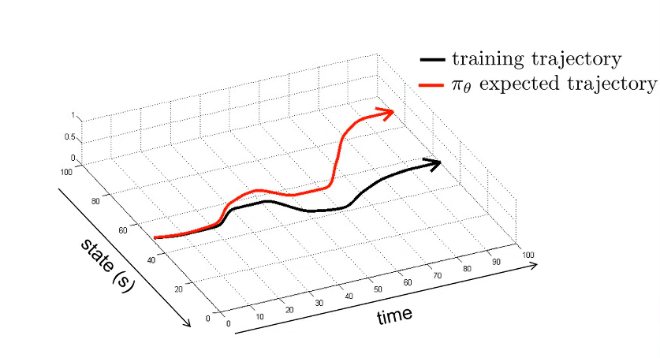
\includegraphics[width=0.4\linewidth,keepaspectratio]{rl49}

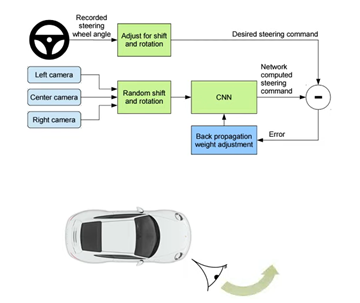
\includegraphics[width=0.4\linewidth,keepaspectratio]{rl50}

\end{center}

Markovian means if we see the same thing twice, we do the same thing twice, regardless of what happened before.


{\tiny (Ref: CS 285 Fall 2020 Deep Reinforcement Learning)}

\end{frame}

%%%%%%%%%%%%%%%%%%%%%%%%%%%%%%%%%%%%%%%%%%%%%%%%%%%%%%%%%%%%%%%%%%%%%%%%%%%%%%%%%%
\begin{frame}[fragile]\frametitle{How to RL?}

\begin{itemize}
\item As we are doing trial and errors, you can not try them in real life (autonomous car?), so a simulation is used to try and train RL, virtual shop, virtual car, etc.
\item Approximately model, key interactions, states, rewards, stochastic inputs, actions, etc.
\item Once proven ok, can be deployed in the real world.
\item So, there are two things in any RL problem
\item Simulation $==$ Environment
\item RL algorithm/Library $==$ Agent.
\end{itemize}
\end{frame}

%%%%%%%%%%%%%%%%%%%%%%%%%%%%%%%%%%%%%%%%%%%%%%%%%%%%%%%%%%%%%%%%%%%%%%%%%%%%%%%%%%
\begin{frame}[fragile]\frametitle{How RL Algorithms work?}

Famous RL Algorithms:
\begin{itemize}
\item Deep Q Network (DQN): Atari video games
\item Proximal Policy Optimization (PPO): DOTA 2
\item Although used in games, RL algorithms are generic and more or less similar.
\end{itemize}

At High level:
\begin{itemize}
\item At start Agent (RL Algorithm) starts with random actions (exploration) to find out their consequent immediate reward and next state. So, Policy here is $\pi(a|s) = random()$ So paths are random. So, low cumulative awards.
\item During exploration, the Agent gathers Experiences, ie $(S,a,S',r_{SS'}^a)$ tuples.
\item Once enough experiences are gathered, they start getting used to decide the next action, with an updated policy $\pi_1$. This is Exploitation and has better Expected cumulative rewards.
\item This goes on, ie more experience, updated policy $\pi_2$ and so on, till the policy does not improve anymore.
\end{itemize}
\end{frame}

%%%%%%%%%%%%%%%%%%%%%%%%%%%%%%%%%%%%%%%%%%%%%%%%%%%%%%%%%%%%%%%%%%%%%%%%%%%%%%%%%%
\begin{frame}[fragile]\frametitle{How RL Algorithms work?}

\begin{center}
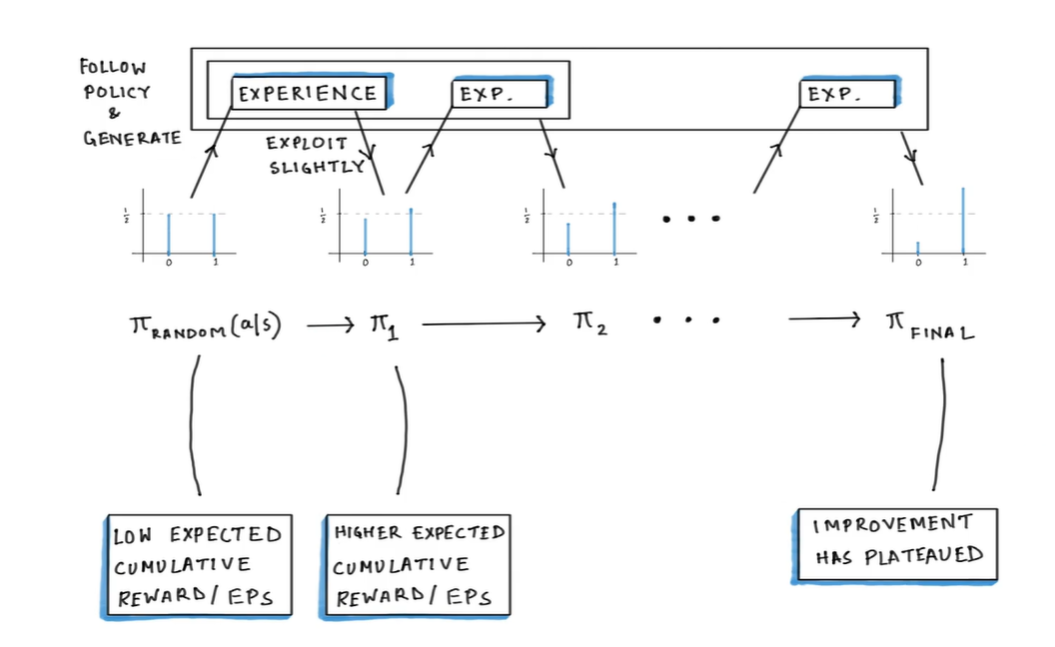
\includegraphics[width=0.8\linewidth,keepaspectratio]{rl62}

{\tiny (Ref: Fast RL course - Dibya Chakraborty)}
\end{center}

\end{frame}


%%%%%%%%%%%%%%%%%%%%%%%%%%%%%%%%%%%%%%%%%%%%%%%%%%%%%%%%%%%%%%%%%%%%%%%%%%%%%%%%%%
\begin{frame}[fragile]\frametitle{How RL Algorithms work?}

\begin{center}
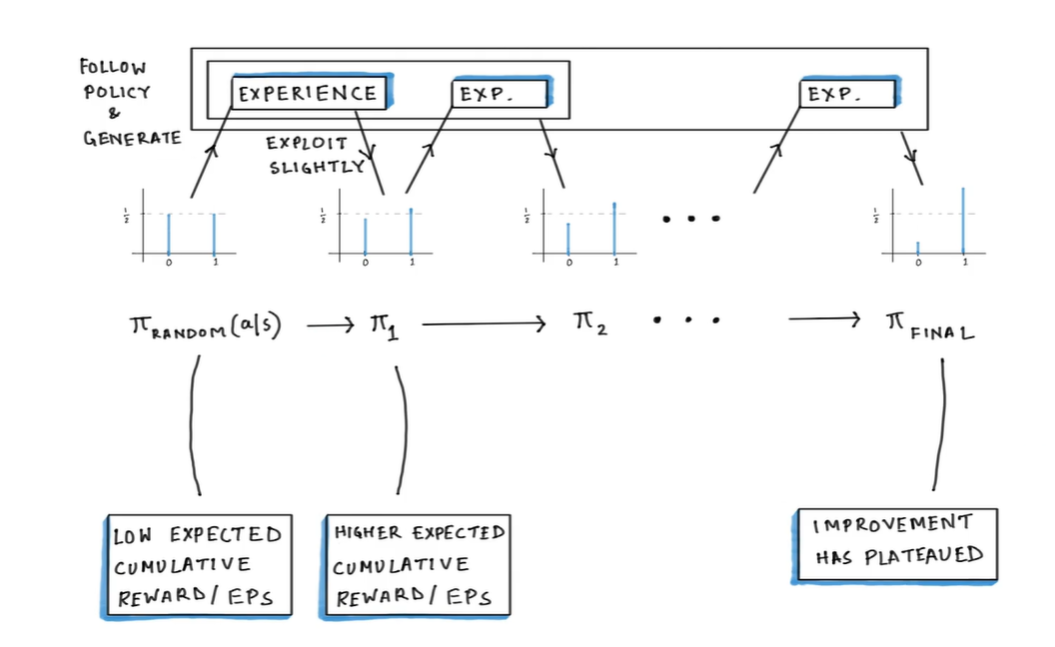
\includegraphics[width=0.4\linewidth,keepaspectratio]{rl62}

{\tiny (Ref: Fast RL course - Dibya Chakraborty)}
\end{center}

\begin{itemize}
\item Note how the final policy is very different from the initial ones, but deltas among neighbors is small.
\item For continuous rewards, there is probability distribution, instead of discrete values.
\item This process is ok for small state spaces, but not for millions, like in Atari game, it goes in millions. 
\item Solution: Deep RL: Neural Network takes state as input and outputs some quantity useful for exploitation.
\item RL Algorithms structure is same but how they update the policy based on experiences, differ.
\end{itemize}
\end{frame}


%%%%%%%%%%%%%%%%%%%%%%%%%%%%%%%%%%%%%%%%%%%%%%%%%%%%%%%%%%%%%%%%%%%%%%%%%%%%%%%%%%
\begin{frame}[fragile]\frametitle{Policy: Actor Critic Method}


\begin{center}
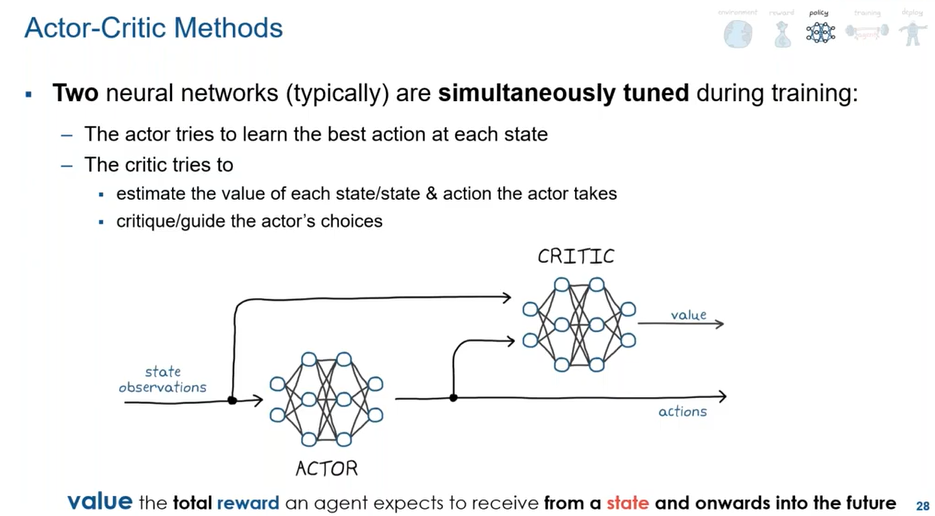
\includegraphics[width=0.9\linewidth,keepaspectratio]{rl80}
\end{center}

{\tiny (Ref: How to Train Your Robot: An Introduction to Reinforcement Learning - Craig Buhr PhD)}

\end{frame}

%%%%%%%%%%%%%%%%%%%%%%%%%%%%%%%%%%%%%%%%%%%%%%%%%%%%%%%%%%%%%%%%%%%%%%%%%%%%%%%%%%
\begin{frame}[fragile]\frametitle{Training: Actor Critic Method}


\begin{center}
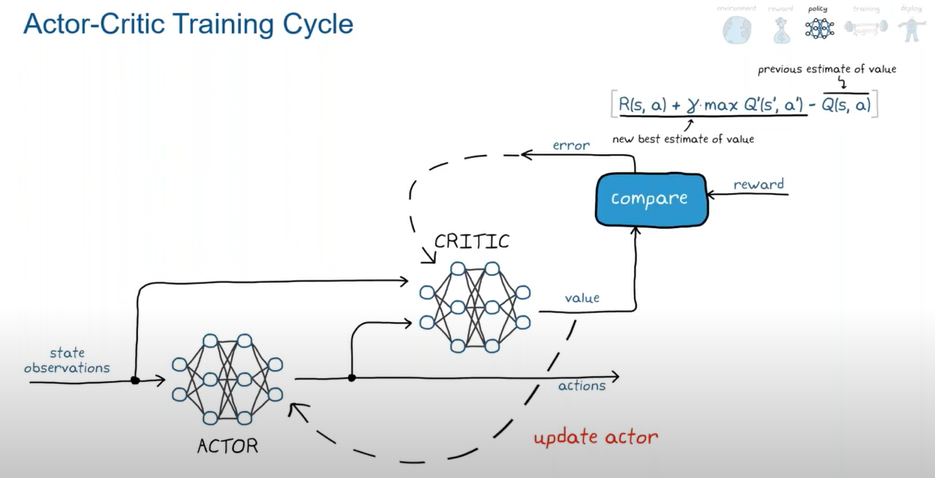
\includegraphics[width=0.9\linewidth,keepaspectratio]{rl81}
\end{center}

{\tiny (Ref: How to Train Your Robot: An Introduction to Reinforcement Learning - Craig Buhr PhD)}

\end{frame}


